%!TEX root=../paper/paper.tex
\chapter{Image Style Recognition Detailed Results}\label{sec:style_appendix}

% \begin{figure}[th]
% \centering
% 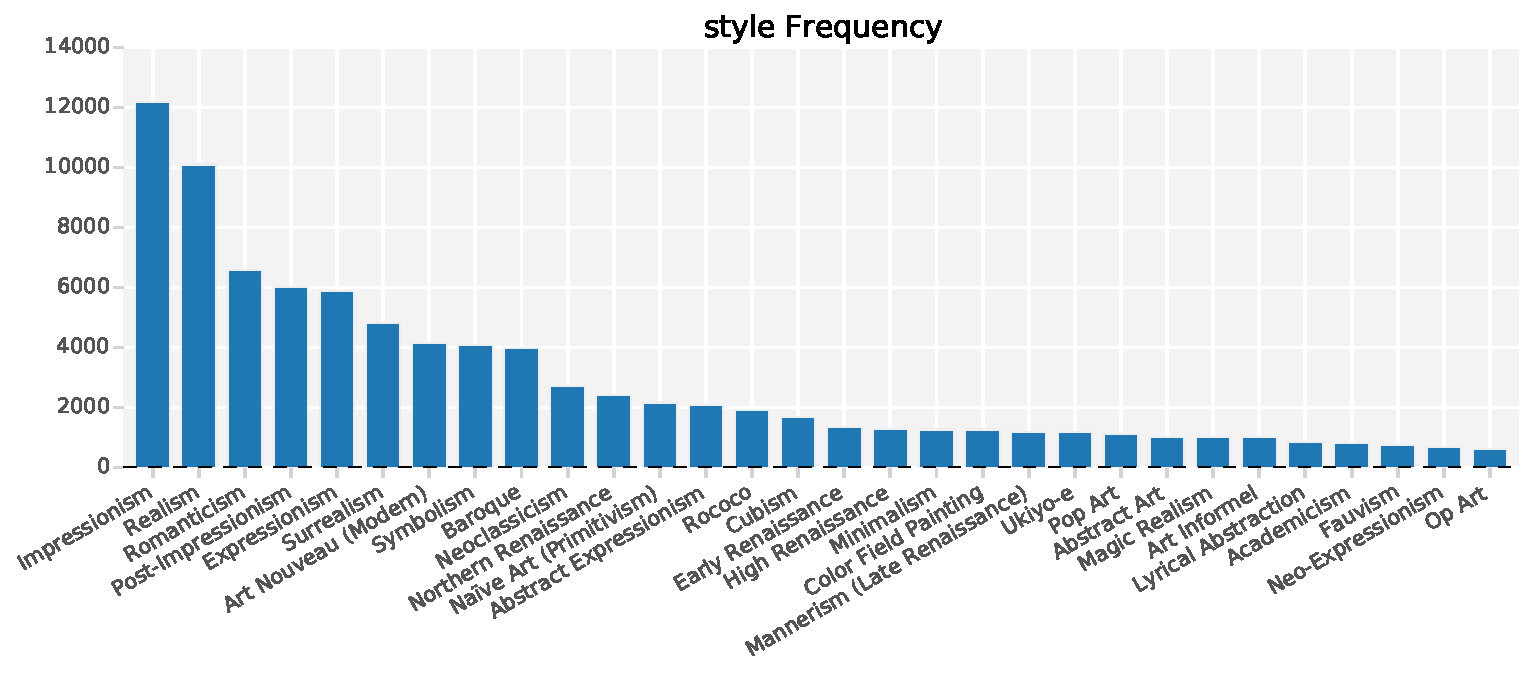
\includegraphics[width=\linewidth]{../style/figures/wikipaintings_style.pdf}\\
% 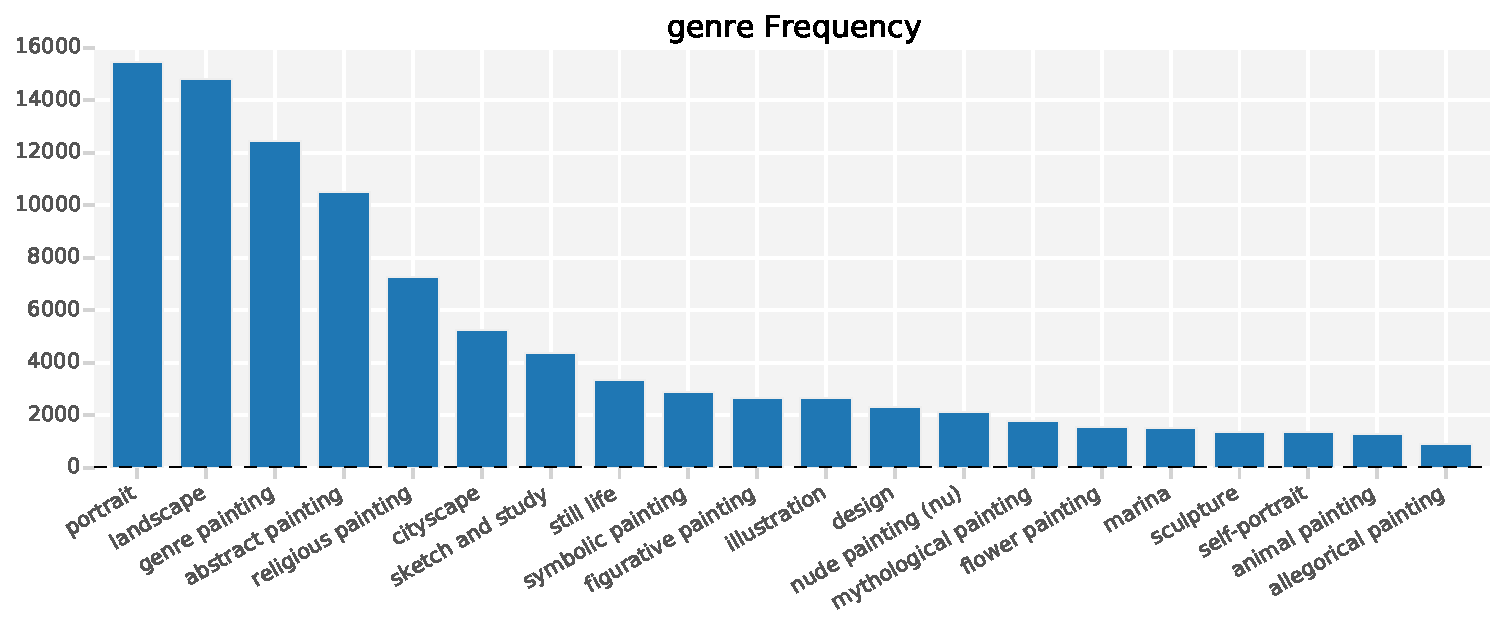
\includegraphics[width=\linewidth]{../style/figures/wikipaintings_genre.pdf}\\
% 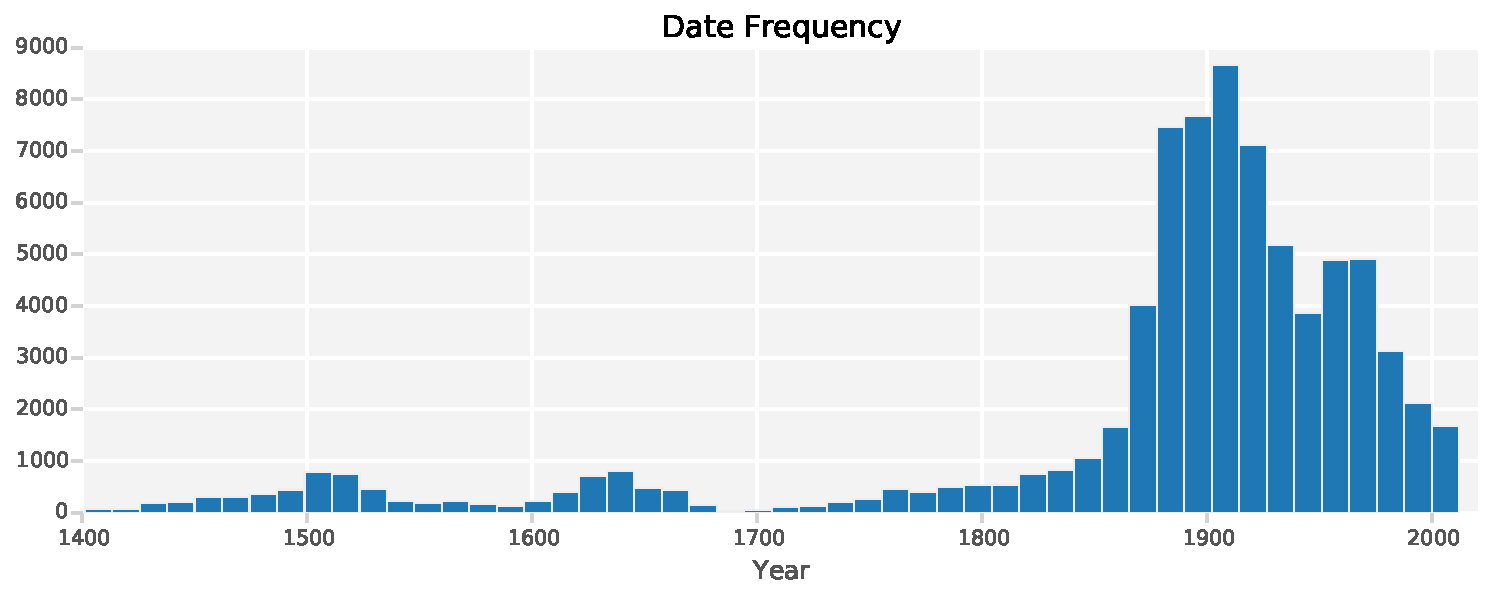
\includegraphics[width=\linewidth]{../style/figures/wikipaintings_date.pdf}
% \caption{Distribution of image style, genre, and date in the Wikipaintings dataset.}
% \label{fig:wikipaintings_data}
% \end{figure}

\begin{table*}[ht!]
\caption{
    All per-class APs on all evaluated features on the AVA Style dataset.
}\label{tab:ava_style_ap_table}
\vspace{1em}
\centering
\small{
\begin{tabular}{lllllrlllll}
\toprule
{}                    & Fusion & DeCAF$_6$ & MC-bit & Murray & L*a*b* & GIST  & Saliency \\
\midrule
Complementary\_Colors & 0.469  & 0.548     & 0.329  & 0.440  & 0.294  & 0.223 & 0.111 \\
Duotones              & 0.676  & 0.737     & 0.612  & 0.510  & 0.582  & 0.255 & 0.233 \\
HDR                   & 0.669  & 0.594     & 0.624  & 0.640  & 0.194  & 0.124 & 0.101 \\
Image\_Grain          & 0.647  & 0.545     & 0.744  & 0.740  & 0.213  & 0.104 & 0.104 \\
Light\_On\_White      & 0.908  & 0.915     & 0.802  & 0.730  & 0.867  & 0.704 & 0.172 \\
Long\_Exposure        & 0.453  & 0.431     & 0.420  & 0.430  & 0.232  & 0.159 & 0.147 \\
Macro                 & 0.478  & 0.427     & 0.413  & 0.500  & 0.230  & 0.269 & 0.161 \\
Motion\_Blur          & 0.478  & 0.467     & 0.458  & 0.400  & 0.117  & 0.114 & 0.122 \\
Negative\_Image       & 0.595  & 0.619     & 0.499  & 0.690  & 0.268  & 0.189 & 0.123 \\
Rule\_of\_Thirds      & 0.352  & 0.353     & 0.236  & 0.300  & 0.188  & 0.167 & 0.228 \\
Shallow\_DOF          & 0.624  & 0.659     & 0.637  & 0.480  & 0.332  & 0.276 & 0.223 \\
Silhouettes           & 0.791  & 0.801     & 0.801  & 0.720  & 0.261  & 0.263 & 0.130 \\
Soft\_Focus           & 0.312  & 0.354     & 0.290  & 0.390  & 0.127  & 0.126 & 0.114 \\
Vanishing\_Point      & 0.684  & 0.658     & 0.685  & 0.570  & 0.123  & 0.107 & 0.161 \\
\midrule
mean                  & 0.581  & 0.579     & 0.539  & 0.539  & 0.288  & 0.220 & 0.152 \\
\bottomrule
\end{tabular}
}
\end{table*}

\begin{table*}[ht!]
\caption{
    All per-class APs on all evaluated features on the Flickr dataset.
}\label{tab:flickr_ap_table}
\vspace{1em}
\centering
\begin{tabular}{llll}
\toprule
{}                     & Fusion x Content & DeCAF$_6$ & MC-bit \\
\midrule
Bokeh                  & 0.288            & 0.253     & 0.248 \\
Bright                 & 0.251            & 0.236     & 0.183 \\
Depth\_of\_Field       & 0.169            & 0.152     & 0.148 \\
Detailed               & 0.337            & 0.277     & 0.278 \\
Ethereal               & 0.408            & 0.393     & 0.335 \\
Geometric\_Composition & 0.411            & 0.355     & 0.360 \\
HDR                    & 0.487            & 0.406     & 0.475 \\
Hazy                   & 0.493            & 0.451     & 0.447 \\
Horror                 & 0.400            & 0.396     & 0.295 \\
Long\_Exposure         & 0.515            & 0.457     & 0.463 \\
Macro                  & 0.617            & 0.582     & 0.530 \\
Melancholy             & 0.168            & 0.147     & 0.136 \\
Minimal                & 0.512            & 0.444     & 0.481 \\
Noir                   & 0.494            & 0.481     & 0.408 \\
Pastel                 & 0.258            & 0.245     & 0.211 \\
Romantic               & 0.227            & 0.204     & 0.185 \\
Serene                 & 0.281            & 0.257     & 0.239 \\
Sunny                  & 0.500            & 0.481     & 0.453 \\
Texture                & 0.265            & 0.227     & 0.229 \\
Vintage                & 0.282            & 0.273     & 0.222 \\
\midrule
mean                   & 0.368            & 0.336     & 0.316 \\
\bottomrule
\end{tabular}
\end{table*}

\begin{table*}[ht!]
\caption{Comparison of Flickr Style per-class accuracies for our method and Mech Turkers.}\label{tab:flickr_vs_mturk}
\centering
\small{
\begin{tabular}{rccc}
\toprule
{}                    & MTurk acc., Flickr g.t. & Our acc., Flickr g.t. & Our acc., MTurk g.t. \\
\midrule
Bright                & 69.10                       & 73.38                     & 73.63 \\
Depth of Field        & 68.92                       & 68.50                     & 81.05 \\
Detailed              & 65.47                       & 75.25                     & 68.44 \\
Ethereal              & 76.92                       & 80.62                     & 77.95 \\
Geometric Composition & 81.52                       & 77.75                     & 80.31 \\
HDR                   & 71.84                       & 82.00                     & 76.96 \\
Hazy                  & 83.49                       & 80.75                     & 81.64 \\
Horror                & 89.85                       & 84.25                     & 81.64 \\
Long Exposure         & 73.12                       & 84.19                     & 76.79 \\
Macro                 & 92.25                       & 86.56                     & 88.39 \\
Melancholy            & 67.77                       & 70.88                     & 71.25 \\
Minimal               & 79.71                       & 83.75                     & 78.57 \\
Noir                  & 81.35                       & 85.25                     & 85.88 \\
Pastel                & 66.94                       & 74.56                     & 75.47 \\
Romantic              & 60.91                       & 68.00                     & 66.25 \\
Serene                & 69.49                       & 70.44                     & 76.80 \\
Sunny                 & 84.48                       & 84.56                     & 79.94 \\
Vintage               & 68.77                       & 75.50                     & 67.80 \\
\midrule
Mean                  & 75.11                       & 78.12                     & 77.15 \\
\end{tabular}
}
\end{table*}

\begin{table*}[ht!]
\caption{Signficant deviations between human and machine accuracies on Flickr Style.}\label{tab:flickr_vs_mturk2}
\centering
\small{
\begin{tabular}{rccc}
\toprule
{}                    & Our acc., Flickr g.t.   & Our acc., MTurk g.t.  & \% change from Flickr to MTurk g.t. \\
\midrule
Vintage               & 75.50                       & 67.80                     & -10.19 \\
Detailed              & 75.25                       & 68.44                     & -9.05 \\
Long Exposure         & 84.19                       & 76.79                     & -8.79 \\
Minimal               & 83.75                       & 78.57                     & -6.18 \\
HDR                   & 82.00                       & 76.96                     & -6.15 \\
Sunny                 & 84.56                       & 79.94                     & -5.46 \\
Serene                & 70.44                       & 76.80                     & 9.03 \\
Depth of Field        & 68.50                       & 81.05                     & 18.32 \\
\toprule
{}                     & Our acc., Flickr g.t. & MTurk acc., Flickr g.t. & Acc. difference \\
\midrule
Horror                 & 84.25                     & 90.42                       & -6.17 \\
Macro                  & 86.56                     & 91.71                       & -5.15 \\
Romantic               & 68.00                     & 61.04                       & 6.96 \\
Pastel                 & 74.56                     & 66.87                       & 7.69 \\
HDR                    & 82.00                     & 72.79                       & 9.21 \\
Long Exposure          & 84.19                     & 73.83                       & 10.35 \\
Detailed               & 75.25                     & 63.30                       & 11.95 \\
\end{tabular}
}
\end{table*}

\begin{table*}[ht!]
\centering
\caption{
    All per-class APs on all evaluated features on the Wikipaintings dataset.
}\label{tab:wikipaintings_ap_table}
\vspace{1em}
\begin{tabular}{llllll}
\toprule
{}                             & Fusion x Content & MC-bit & DeCAF$_6$  \\
\midrule
Abstract\_Art                  & 0.341            & 0.314  & 0.258      \\
Abstract\_Expressionism        & 0.351            & 0.340  & 0.243      \\
Art\_Informel                  & 0.221            & 0.217  & 0.187      \\
Art\_Nouveau\_(Modern)         & 0.421            & 0.402  & 0.197      \\
Baroque                        & 0.436            & 0.386  & 0.313      \\
Color\_Field\_Painting         & 0.773            & 0.739  & 0.689      \\
Cubism                         & 0.495            & 0.488  & 0.400      \\
Early\_Renaissance             & 0.578            & 0.559  & 0.453      \\
Expressionism                  & 0.235            & 0.230  & 0.186      \\
High\_Renaissance              & 0.401            & 0.345  & 0.288      \\
Impressionism                  & 0.586            & 0.528  & 0.411      \\
Magic\_Realism                 & 0.521            & 0.465  & 0.428      \\
Mannerism\_(Late\_Renaissance) & 0.505            & 0.439  & 0.356      \\
Minimalism                     & 0.660            & 0.614  & 0.604      \\
Nave\_Art\_(Primitivism)       & 0.395            & 0.425  & 0.225      \\
Neoclassicism                  & 0.601            & 0.537  & 0.399      \\
Northern\_Renaissance          & 0.560            & 0.478  & 0.433      \\
Pop\_Art                       & 0.441            & 0.398  & 0.281      \\
Post-Impressionism             & 0.348            & 0.348  & 0.292      \\
Realism                        & 0.408            & 0.309  & 0.266      \\
Rococo                         & 0.616            & 0.548  & 0.467      \\
Romanticism                    & 0.392            & 0.389  & 0.343      \\
Surrealism                     & 0.262            & 0.247  & 0.134      \\
Symbolism                      & 0.390            & 0.390  & 0.260      \\
Ukiyo-e                        & 0.895            & 0.894  & 0.788      \\
\midrule
mean                           & 0.473            & 0.441  & 0.356      \\
\bottomrule
\end{tabular}
\end{table*}

\begin{table*}
\caption{
    Per-class accuracies on the Wikipaintings dataset, using the MC-bit feature.
}\label{tab:wp_accuracies}
\vspace{1em}
\centering
\begin{tabular}{lrlr}
\toprule
\textbf{Style} & \textbf{Accuracy} & \textbf{Style} & \textbf{Accuracy} \\
\midrule
Symbolism                    &         71.24 & Impressionism                &         82.15 \\
Expressionism                &         72.03 & Northern Renaissance         &         82.32 \\
Art Nouveau (Modern)         &         72.77 & High Renaissance             &         82.90 \\
Nave Art (Primitivism)       &         72.95 & Mannerism (Late Renaissance) &         83.04 \\
Surrealism                   &         74.44 & Pop Art                      &         83.33 \\
Post-Impressionism           &         74.51 & Early Renaissance            &         84.69 \\
Romanticism                  &         75.86 & Abstract Art                 &         85.10 \\
Realism                      &         75.88 & Cubism                       &         86.85 \\
Magic Realism                &         78.54 & Rococo                       &         87.33 \\
Neoclassicism                &         80.18 & Ukiyo-e                      &         93.18 \\
Abstract Expressionism       &         81.25 & Minimalism                   &         94.21 \\
Baroque                      &         81.45 & Color Field Painting         &         95.58 \\
Art Informel                 &         82.09 &                              &               \\
\bottomrule
\end{tabular}
\end{table*}

% \begin{figure*}[ht!]
% \centering
% 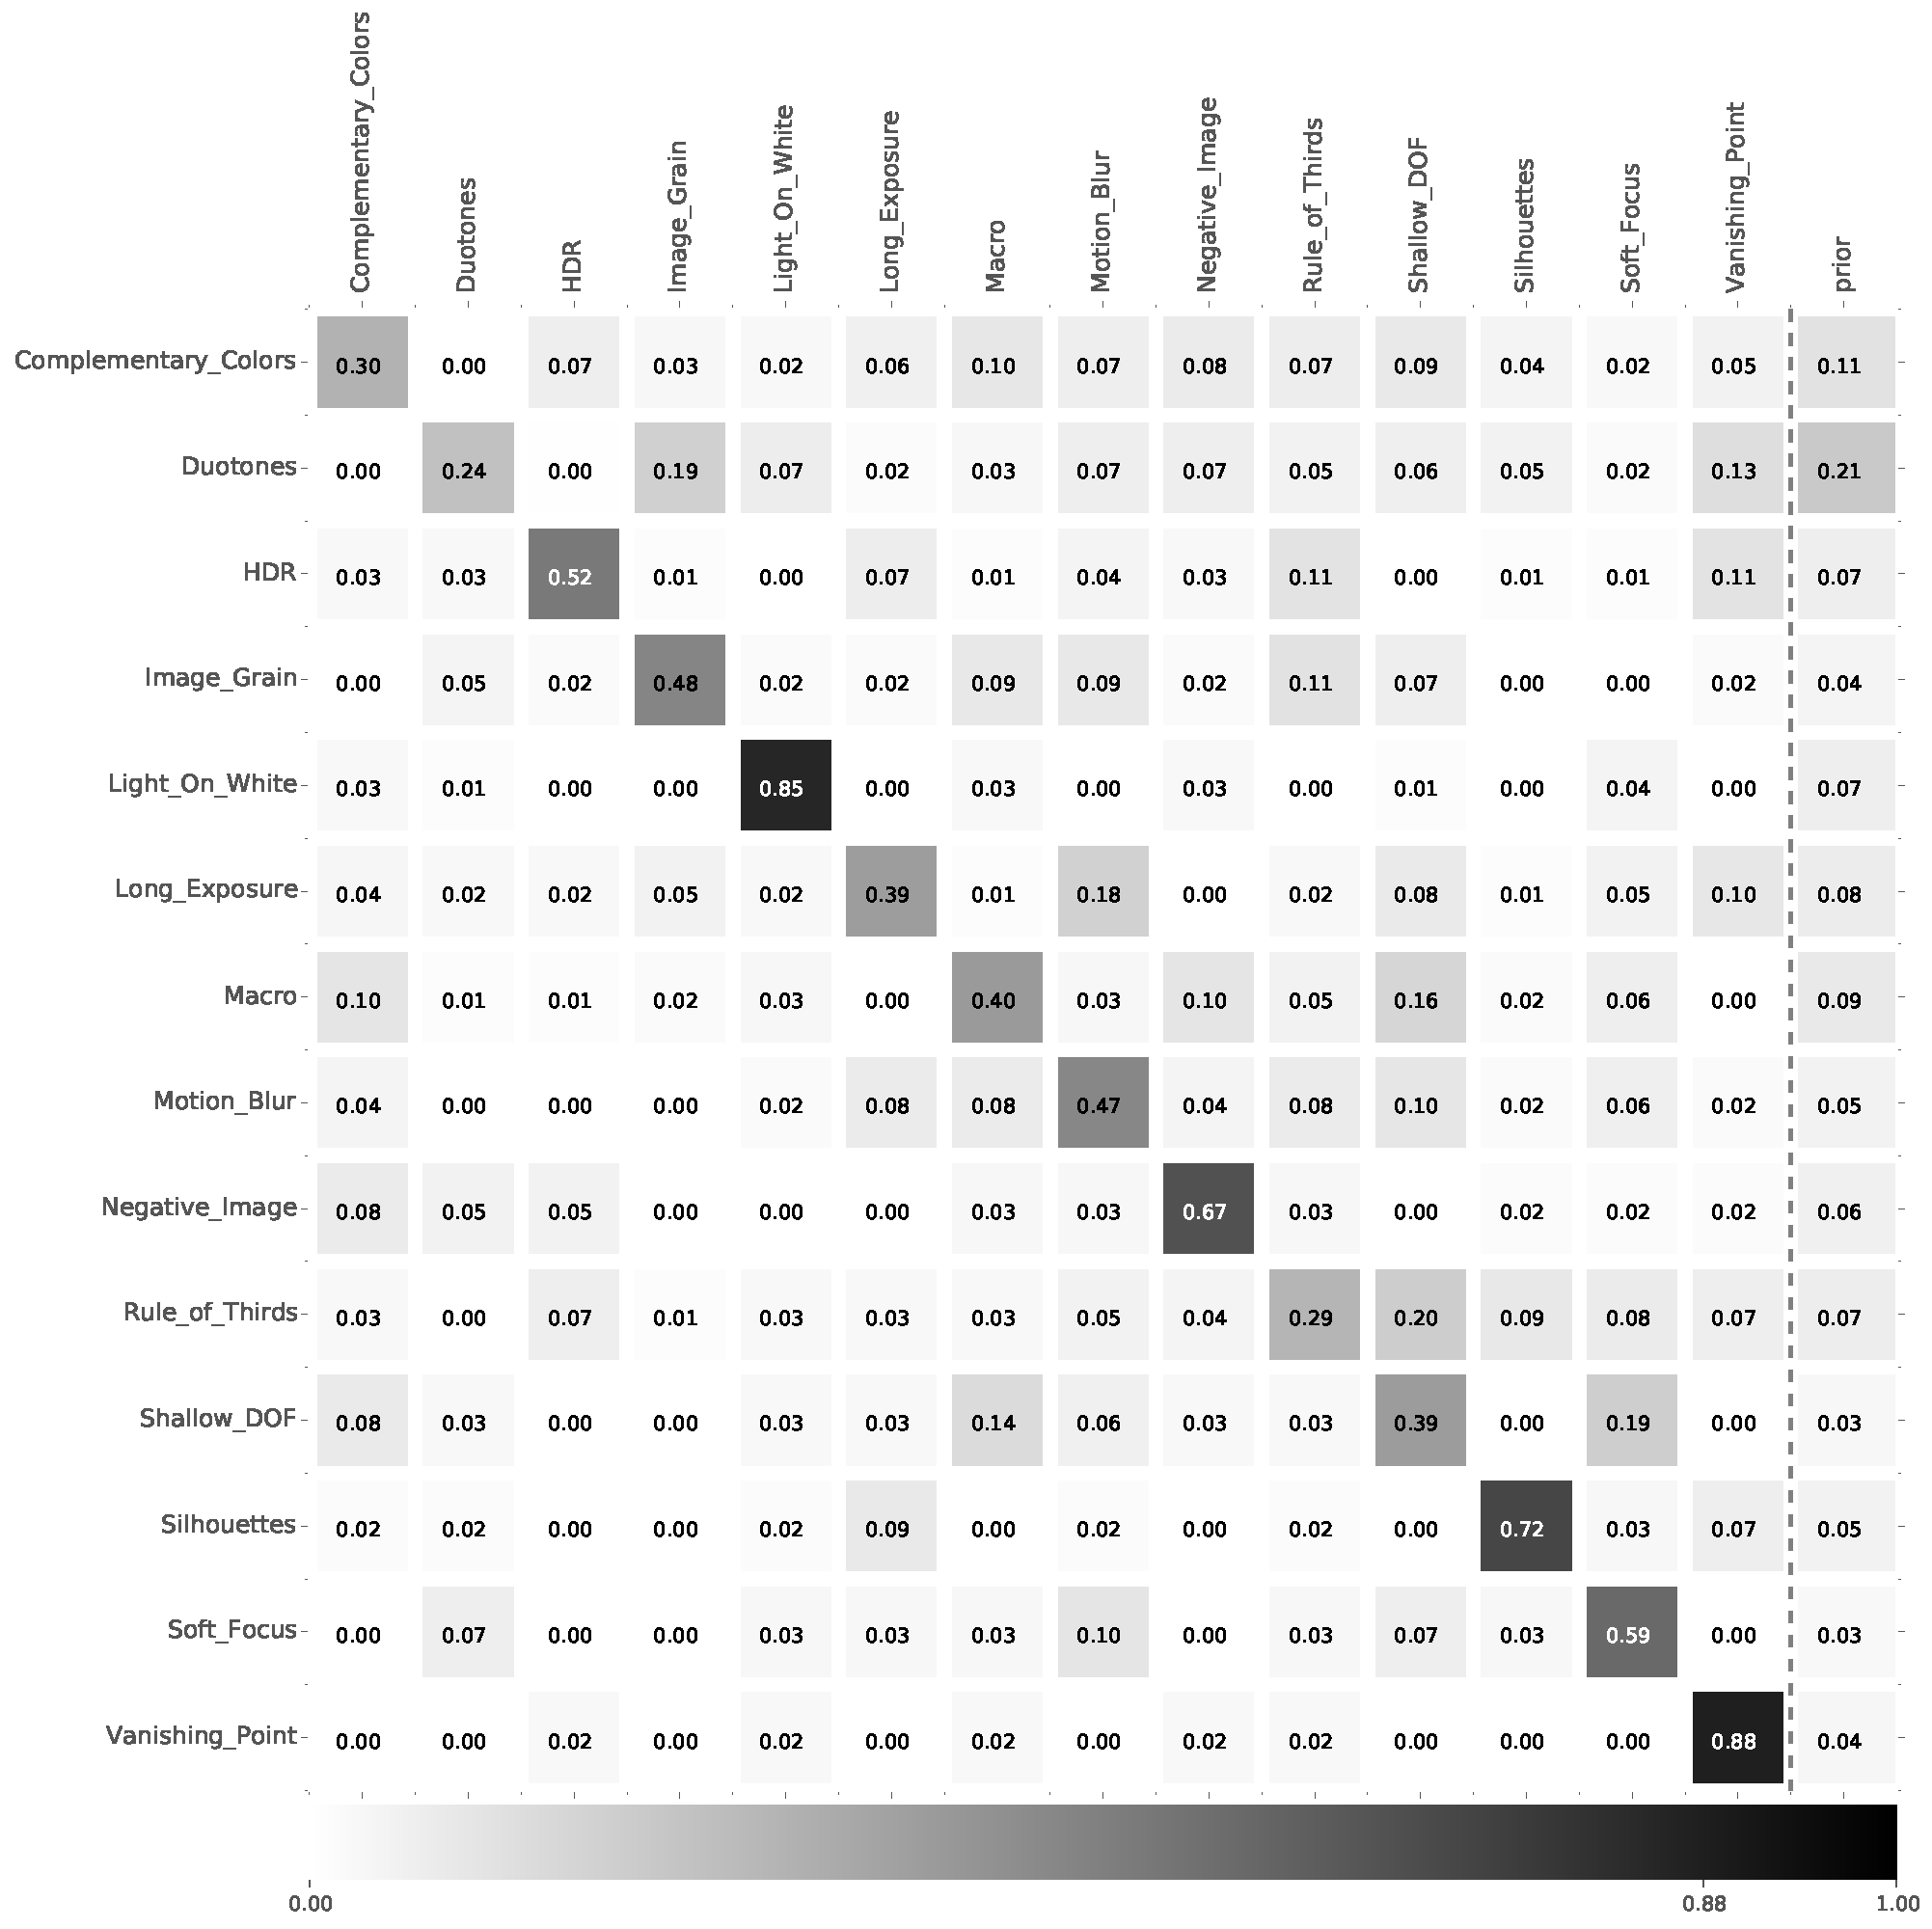
\includegraphics[width=\linewidth]{../style/figures/evaluation/ava_style_conf.pdf}
% \caption
% [Confusion matrix of our best classifier on the AVA Style dataset.]
% {
% Confusion matrix of our best classifier (\mbox{Late-fusion $\times$ Content}) on the AVA Style dataset.
% The right-most ``prior'' column reflects the distribution of ground-truth labels in the test set.
% The confusions are mostly understandable: ``Soft Focus'' vs. ``Motion Blur'' for example.
% }
% \label{fig:ava_style_conf}
% \end{figure*}

\begin{figure*}[ht!]
\centering
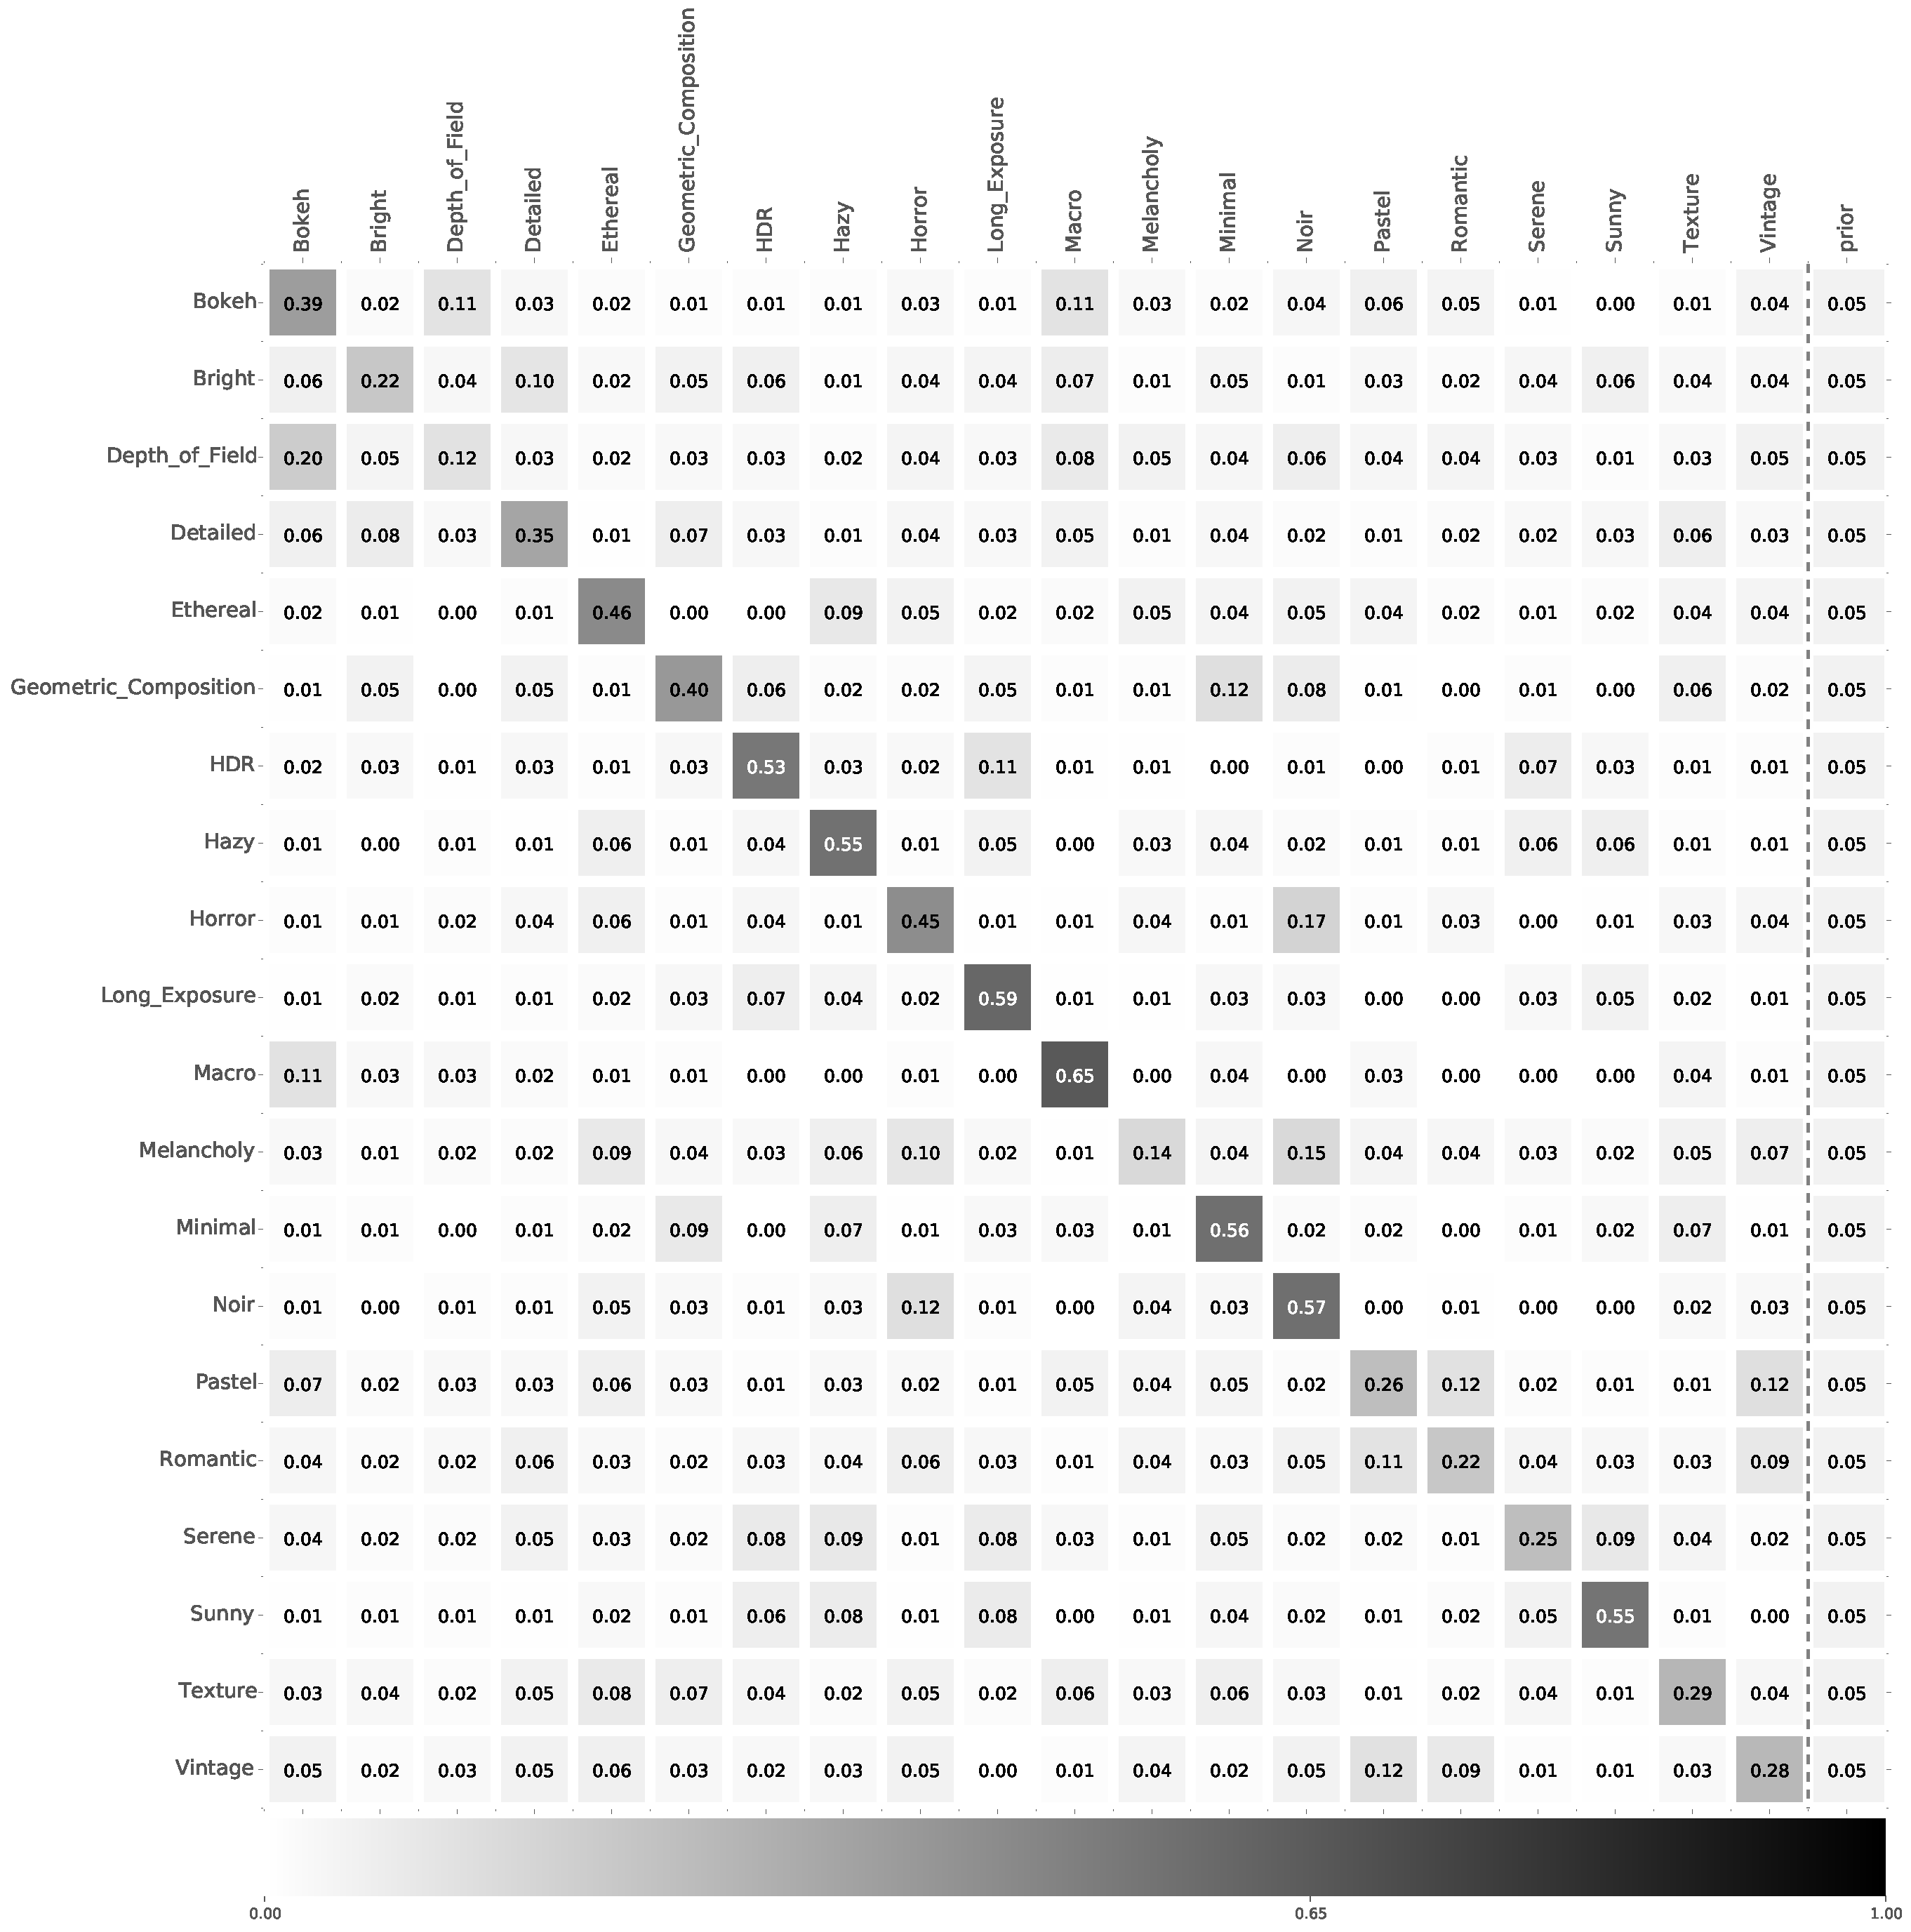
\includegraphics[width=1\linewidth]{../style/figures/evaluation/flickr_conf.pdf}
\caption
[Confusion matrix of our best classifier on the Flickr dataset.]
{Confusion matrix of our best classifier (\mbox{Late-fusion $\times$ Content}) on the Flickr dataset.}
\label{fig:flickr_conf}
\end{figure*}

\begin{figure*}[ht!]
\centering
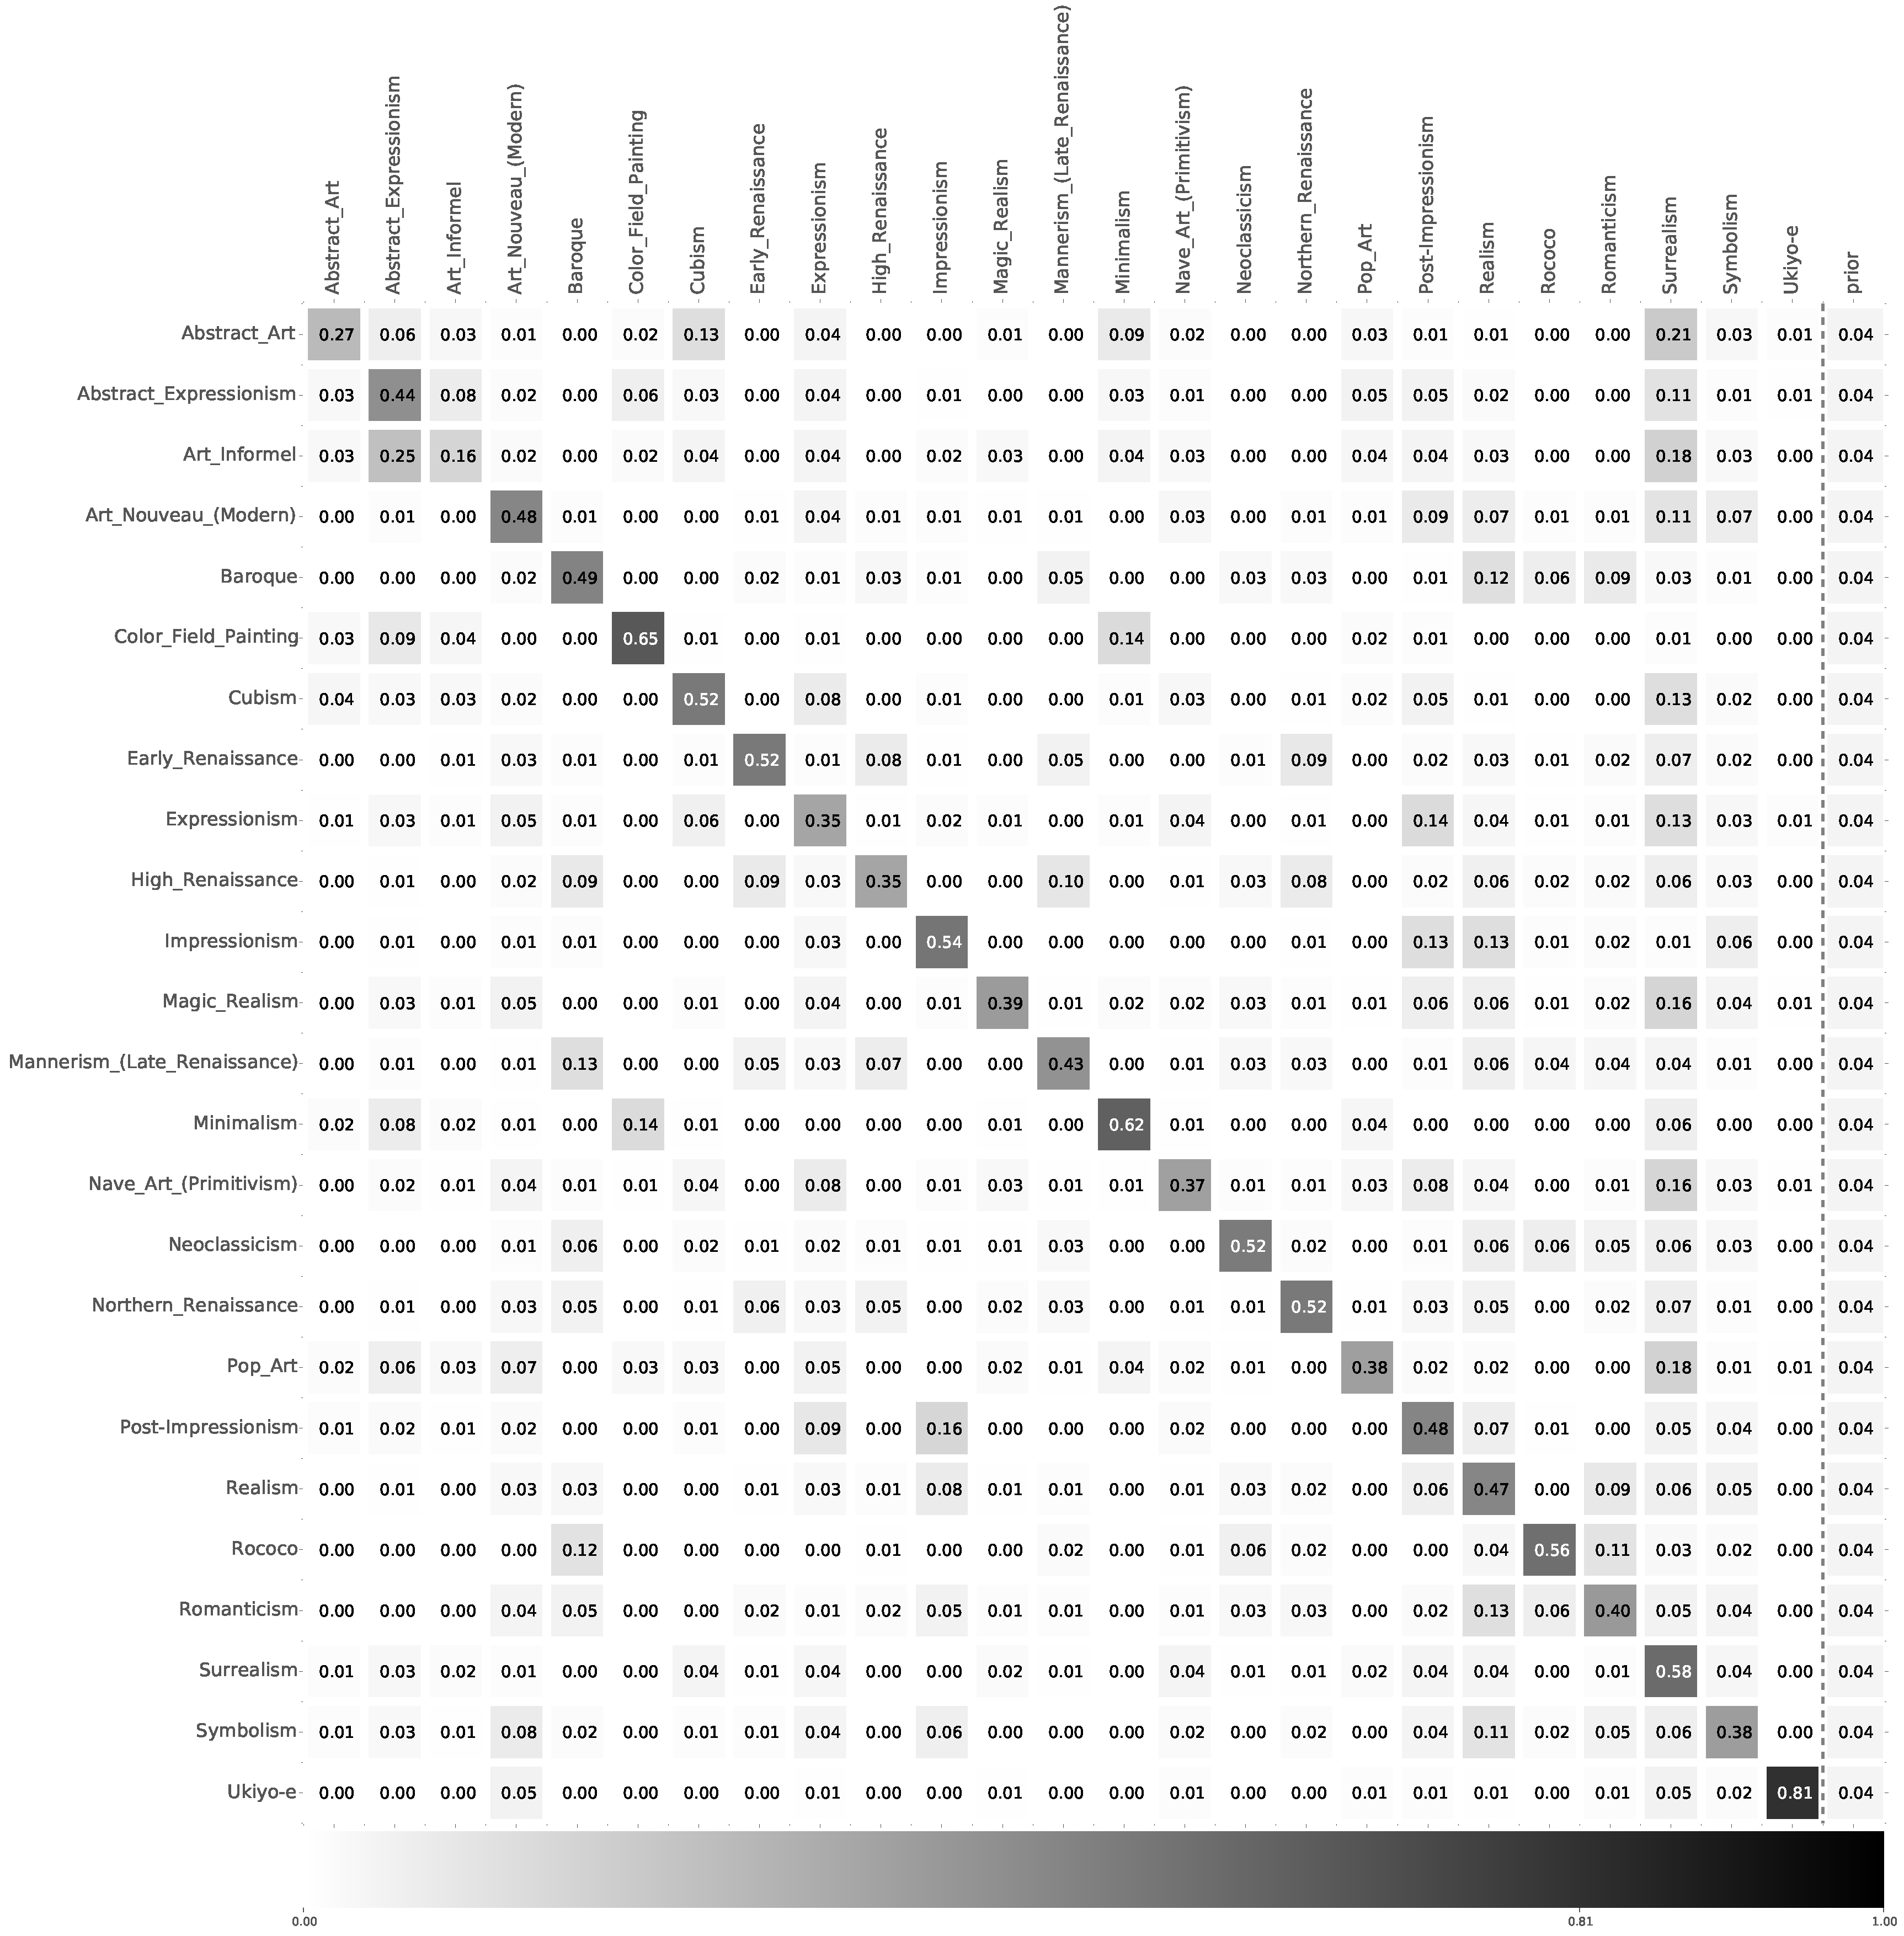
\includegraphics[width=1\linewidth]{../style/figures/evaluation/wikipaintings_conf.pdf}
\caption
[Confusion matrix of our best classifier on the Wikipaintings dataset.]
{Confusion matrix of our best classifier (\mbox{Late-fusion $\times$ Content}) on the Wikipaintings dataset.}
\label{fig:wp_conf}
\end{figure*}
